\documentclass[11pt,a4paper]{article}
\usepackage[margin=2.2cm]{geometry}
\usepackage{booktabs}
\usepackage{graphicx}
\usepackage{amsmath}
\usepackage{float}
\usepackage[hidelinks]{hyperref}

\title{Assignment 7: Graph Neural Networks + State Space Models}
\author{}
\date{}

\begin{document}
\maketitle
\vspace{-1.5cm}

All experiments use the Fashion Product Images (Small) dataset from Kaggle (44,391 products, 5 master categories). Each product's \texttt{productDisplayName} is used as input text, and \texttt{masterCategory} (Accessories, Apparel, Footwear, Free Items, Personal Care) is the classification target. The vocabulary contains 4,807 words; sequences are capped at 20 tokens. Data is split 80/20 into 35,512 training and 8,879 test samples.

\section{Part A: GNN Baseline}

\textbf{A1 -- Text graph construction.} Each product name is converted to a word graph where nodes are word tokens (embedded via a learnable lookup table, 64-d) and edges connect consecutive words bidirectionally.

\textbf{A2 -- Message passing layer (from scratch).} We implement a single message passing layer with three steps: (1)~\emph{message}: transform each neighbour's features via a linear projection $\mathbf{m}_{j \to i} = W_\text{msg} \, \mathbf{h}_j$; (2)~\emph{aggregate}: sum all incoming messages $\mathbf{m}_i = \sum_{j \in \mathcal{N}(i)} \mathbf{m}_{j \to i}$; (3)~\emph{update}: combine with the node's own features $\mathbf{h}_i' = \text{ReLU}(W_\text{upd} [\mathbf{h}_i \| \mathbf{m}_i])$.

\textbf{A3 -- Pooling and classifier.} After message passing, we apply mean pooling over all node features to get a single graph-level representation, followed by a linear classifier.

\textbf{A4 -- Training.} Cross-entropy loss with Adam optimiser ($\text{lr}=10^{-3}$), cosine annealing schedule, 20 epochs.

\section{Part B: SSM Baseline (Mamba)}

The SSM-only model replaces the graph structure with a sequential state space model. Token embeddings are fed through a Mamba layer (selective state space model with $d_\text{state}=16$, $d_\text{conv}=4$, expand factor 2), which processes the sequence left-to-right and produces contextualised features. Masked mean pooling (ignoring padding) produces a fixed-size representation for the classifier.

Mamba is significantly faster than the GNN because it processes the entire batch as a tensor operation (87.6s total) versus the GNN's per-sample graph construction loop (653.7s). This $7.5\times$ speedup is a key practical advantage of SSMs over GNNs for sequential data.

\section{Part C: Hybrid SSM + GNN}

The hybrid model chains both approaches: token embeddings first pass through the Mamba SSM to produce contextualised features (capturing sequential/positional information), then the word graph is constructed on the same tokens and one message passing layer operates on the SSM-enriched node features. This allows the GNN to work with features that already encode sequential context rather than raw embeddings.

\section{Part D: Experiments}

\begin{table}[H]
\centering
\begin{tabular}{lccc}
\toprule
Model & Params & Best Test Acc & Time \\
\midrule
D1: GNN-only & 320,325 & 0.9950 & 654s \\
D2: SSM-only (Mamba) & 340,613 & 0.9952 & 88s \\
D3: Hybrid SSM+GNN & 352,965 & 0.9952 & 642s \\
\bottomrule
\end{tabular}
\caption{Comparison of all three architectures on Fashion Product classification.}
\end{table}

\begin{figure}[H]
\centering
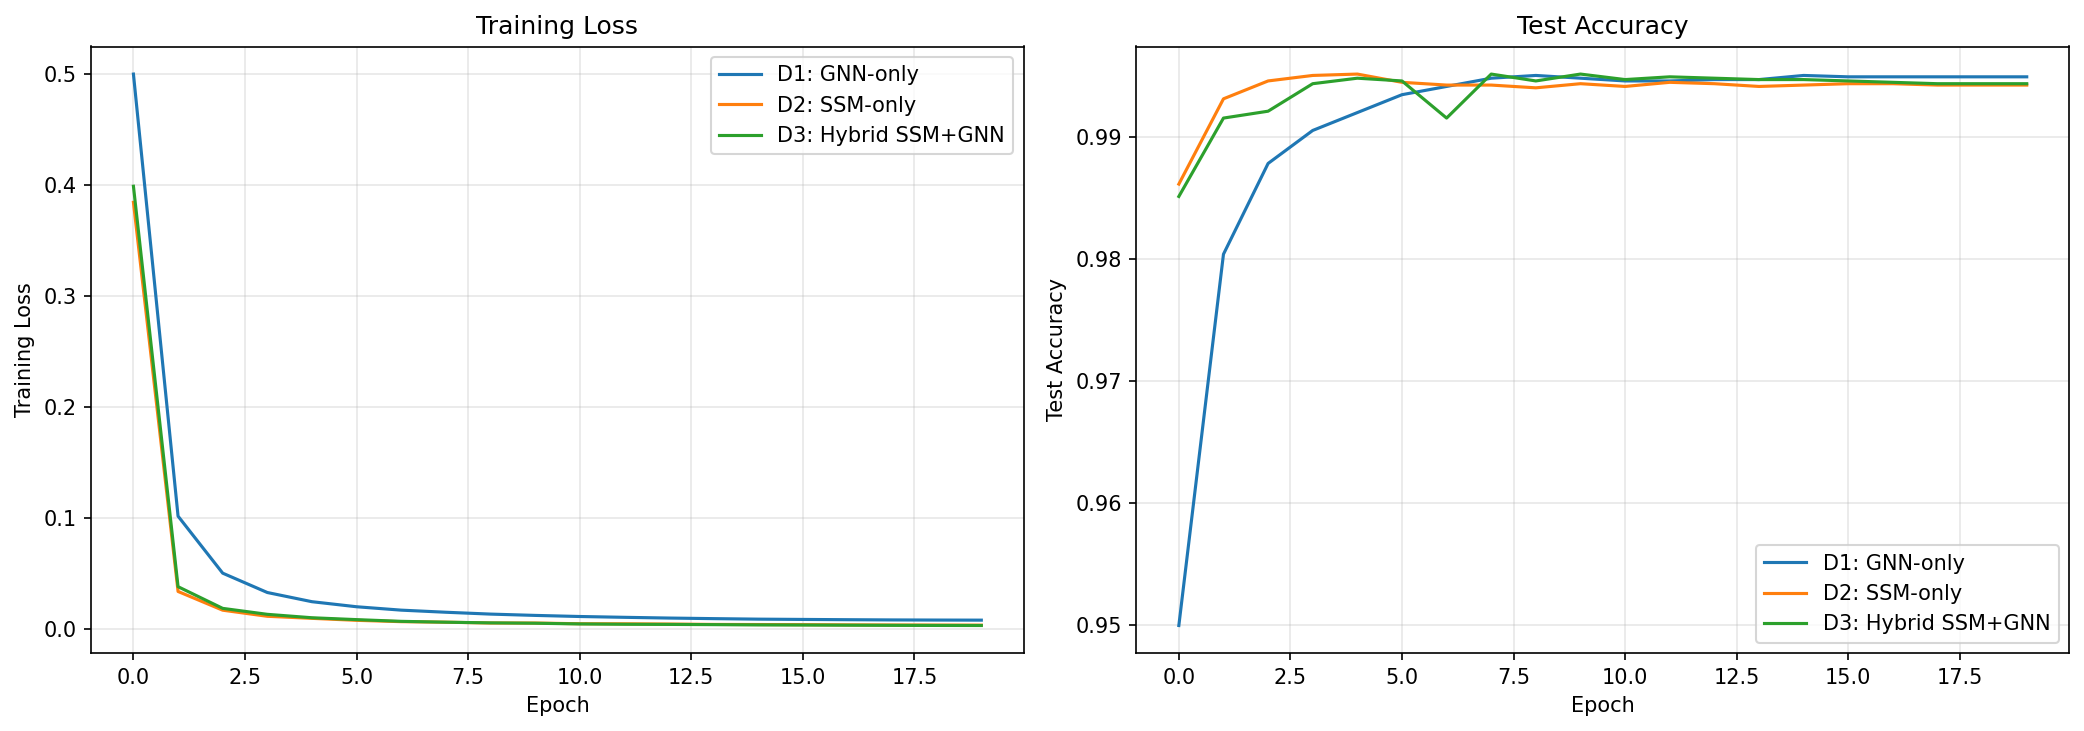
\includegraphics[width=0.95\textwidth]{training_curves.png}
\caption{Training loss and test accuracy curves for all three models.}
\end{figure}

All three models converge to nearly identical accuracy ($\sim$99.5\%), which reflects the relative simplicity of the classification task -- product names often contain the category directly (e.g., ``Nike Men Blue Tshirt'' clearly maps to Apparel). The key differences are in convergence speed and computational cost:

The \textbf{GNN-only} model converges slower initially (95.0\% at epoch 1 vs 98.6\% for SSM) because raw word embeddings without positional context make the first message passing step less informative. However, the graph structure eventually captures sufficient word-neighbourhood information.

The \textbf{SSM-only} model converges fastest because Mamba's selective state space mechanism efficiently captures sequential patterns in the token stream, and batched tensor operations avoid the per-sample loop required by the GNN.

The \textbf{hybrid model} matches the SSM's final accuracy but does not surpass it, because on this dataset the sequential information captured by Mamba is already sufficient for near-perfect classification. The additional message passing layer adds computational cost (642s vs 88s) without measurable benefit. On more complex tasks where graph topology carries information beyond sequential order (e.g., dependency parse graphs, molecular graphs), the hybrid approach would likely show a clearer advantage.

\end{document}
